\chapter{The k-Means Clustering Algorithm}\label{chapter:kmeans}

In this chapter the data mining algorithm k-Means is presented. K-means is a well-studied clustering algorithm, partitioning a data set into $k$ clusters, where all data objects within a cluster are similar to each other and dissimilar to the data objects in the other clusters. The goal is to find the best clustering, minimizing the total distance between each data point and its assigned center. While the solution to that problem is NP-hard~\parencite{nphard1}\parencite{nphard2}, there are several heuristics, in particular the Lloyd algorithm~\parencite{Lloyd82}, which is a local search solution to this problem.

\section{Motivation}
 
We decided to use k-Means as proof-of-concept algorithm for data mining in the HyPer database because it is an algorithm widely used and very popular. In fact, a survey of clustering data mining techniques in 2002 states that the algorithm~\enquote{is by far the most popular clustering algorithm used in scientific and industrial applications}~\parencite{berkhin2002survey}. K-Means is also part of the 10 top data mining algorithms identified by the IEEE International Conference on Data Mining (ICDM)~\parencite{top10}, next to other famous algorithms such as the SVM~\parencite{svm} and the PageRank~\parencite{pagerank} algorithm. 
\\
Since the algorithm is popular and easy to understand, k-Means is suitable as first implementation of a data mining algorithm on HyPer. To our best knowledge, all major data mining tools are implementing k-Means, which is a basic requirement regarding the comparability among existing tools and our own implementation. Hence, the running time is a good measurement for comparing the performance; the cluster compactness, i.e. the sum of squared errors, can be used as general criterion for the formal correctness of the implementation. 
Parts of k-Means can be executed in parallel, and since HyPer supports parallel computation, it will be interesting to evaluate how a single-threaded execution of k-Means performs against a multi-threaded computation. In fact, we are expecting tremendous performance gains executing k-Means in parallel on a multi core machine.

\section{The Lloyd Algorithm}

In this section we discuss the Lloyd algorithm~\parencite{Lloyd82}, usually referred as k-Means in literature and in this work as well. Formally, the k-Means problem and the k-Means algorithm are described the following: For a given integer $k$ and a data set of $n$ data points $X \subset  \mathbb{R}^d$, choose $k$ centers $C$ to minimize the sum of squared error function,
\begin{equation*}
sse = \Sigma_{x \in X} min_{c \in C} ||x - c||^2.
\end{equation*}
After finding these center points, each data point is assigned to its closest center which forms the clustering. 
\\ 
Solving such a problem is NP-hard, however Lloyd proposes a local search solution usually resulting in good groupings. The algorithm starts with $k$ arbitrary center points, typically chosen at random from the data points. Then, each data point is assigned to the closest center using the euclidean distance. After assigning each data point to its closest center, the centers get updated, i.e. the new center is the mean coordinate of all the data points assigned to this center. Then the next iteration begins, assigning the data points again, now to the updated centers. This continues until the process stabilizes and the algorithm converges.
\\
Formally, the k-Means algorithm is described then the following:

\begin{enumerate} 
\item Arbitrarily choose $k$ centers $C = \{c_1, c_2, \cdots, c_k\}$ uniformly at random from $X$.
\item For each $i \in \{1, \cdots, k\}$, set the cluster $C_i$ to be the set of points in $X$ that are closer to cluster $c_i$ than to any other cluster $c_j$ for all $j \neq i$.
\item For each $i \in \{1, \cdots, k\}$, set $c_i$ as the center of all points assigned to $C_i$: 

\begin{equation*}
c_i = \frac{1}{|C_i|} \Sigma_{x \in C_i} x.
\end{equation*}

\item Repeat Steps 2 and 3 until $C$ no longer changes, i.e. the algorithm converges.
\end{enumerate}

This simple algorithm terminates in practice very fast and provides mostly good results. However, the clustering can be arbitrarily bad for specific data sets. Therefore, MacQueen~\parencite{macqueen1967some} and Hartigan and Wong~\parencite{hartigan1979algorithm} propose improvements over the Lloyd algorithm, often leading to a faster convergence. Since the goal of this work is to demonstrate k-Means as a proof-of-concept implementation on HyPer, and since most tools, such as R and Julia, are implementing the Lloyd algorithm, we decided use the Lloyd algorithm in the remainder of this work. 

\section{An Example of the k-Means Algorithm}

In this section the k-Means algorithm is presented by a made-up example for deeper understanding. Our example data set consists of five data points with two dimensions: $x_1(3,9), x_2(2,5), x_3(5,8), x_4(7,5), x_5(4,2)$. This data will be clustered using the k-Means algorithm with $k = 2$, i.e. we are searching for two clusters in the data set. First, the algorithm starts with an initialization phase: Randomly, we choose two instances as initial center points. In this example, these data points are $c_1(3,9)$ and $c_2(4,2)$. 
\\
Next, we begin the first iteration of the k-Means algorithm and compute the euclidean distance from each data point to $c_1$ and to $c_2$. Each data point is then assigned to the closest cluster, as shown in~\autoref{tab:kmeans_iter_1}. After Iteration 1, the data points $x_1$ and $x_3$ are closer to $c_1$ and therefore assigned to Cluster $C_1$, while the data points $x_2$, $x_4$ and $x_5$ belong to Cluster $C_2$.

\begin{table}[htsb]
\caption[Computations in Iteration 1]{Computations in Iteration 1.}\label{tab:kmeans_iter_1}
\centering
\begin{tabular}{l l l l}
\toprule
  Data Point & distance to $c_1(3,9)$ & distance to $c_2(4,2)$ & Cluster \\
\midrule
    $x_1(3,9)$ & 0.00 & 7.07 & $C_1$ \\
    $x_2(2,5)$ & 4.12 & 3.61 & $C_2$ \\
    $x_3(5,8)$ & 2.24 & 6.08 & $C_1$ \\
    $x_4(7,5)$ & 5.66 & 4.24 & $C_2$ \\
    $x_5(4,2)$ & 7.07 & 0.00 & $C_2$ \\
\bottomrule
\end{tabular}
\end{table}

Now, the centers have to be recalculated as the mean of all assigned data points. The result are the updated center points $c_1(4,8.5)$ and $c_2(4.33,4)$. These are used to compute the distances again for each data point in Iteration 2 as shown in~\autoref{tab:kmeans_iter_2}. As the center points have changed, the distances to the centers are different and data points could be assigned to new clusters. In our made-up example the data points are assigned to the same clusters as after Iteration 1, i.e. no assignment changed. Therefore the algorithm converges and we have found the result.~\autoref{fig:kmeans_example} depicts the two clusters. Cluster $C_1$ with the center point $c_1$ is marked by blue data points and is positioned on the top of the chart, while Cluster $C_2$ with the center point $c_2$ is a broader cluster from the middle of the chart to the bottom.

\begin{table}[htsb]
  \caption[Computations in Iteration 2]{Computations in Iteration 2.}\label{tab:kmeans_iter_2}
  \centering
  \begin{tabular}{l l l l}
    \toprule
      Data Point & distance to $c_1(4,8.5)$ & distance to $c_2(4.33,4)$ & Cluster \\
    \midrule
        $x_1(3,9)$ & 1.12 & 5.17 & $C_1$ \\
        $x_2(2,5)$ & 4.03 & 2.54 & $C_2$ \\
        $x_3(5,8)$ & 1.12 & 4.06 & $C_1$ \\
        $x_4(7,5)$ & 4.61 & 2.85 & $C_2$ \\
        $x_5(4,2)$ & 6.50 & 2.02 & $C_2$ \\
    \bottomrule
  \end{tabular}
\end{table}


\begin{figure}[htsb]
  \centering
  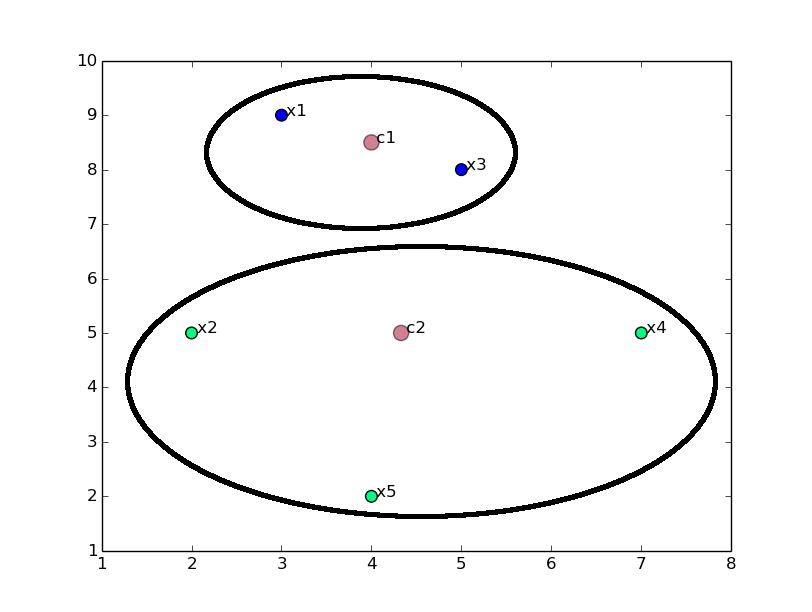
\includegraphics[scale=0.5, trim="0cm 1cm 0cm 0cm"]{figures/kmeans_example2}
  \caption[K-Means Example Clustering]{K-Means Example Clustering.}\label{fig:kmeans_example}
\end{figure}

In this section a made-up example showed the phases of the k-Means algorithm in depth. These fundamentals help us to get a better understanding in Chapter~\ref{chapter:implementation}, when we discuss the implementation details of k-Means as HyPer operator.



\section{The k-Means++ Initialization Strategy}\label{section:kmeans_init}

Even though the Lloyd algorithm provides good results in practice, the resulting clustering can be arbitrarily bad for some data sets. Particularly, the random choosing of the initial cluster centers can lead to a bad grouping which cannot be changed during the clustering process. Therefore,~\cite{kmeans++} proposes a variation to the k-Means initialization strategy, called k-Means++. The centers are still chosen randomly from the data points, but the data points are weighted according to their distance from the closest, already chosen center. Hence, the probability of choosing data points as center that are far away from each other increases, leading to enhancements in speed and accuracy of the clustering.
\\
Formally, k-Means++ can be described the following:
Let $D(x)$ be the shortest distance from a data point to the closest, already picked center.

\begin{enumerate} 
\item Take the first center $c_1$, chosen uniformly at random from $X$.
\item The next center $c_i$ is chosen from $x \in X$ with the probability 

\begin{equation*}
\frac {D(x)^2} {\Sigma_{x \in X} D(x)^2}.
\end{equation*}
This weighting is called the $D^2$ weighting.

\item Repeat Step 2 until all $k$ centers are selected.
\item Continue as in the standard k-Means algorithm.
\end{enumerate}

Many clustering tools implement a k-Means++ initialization strategy for k-Means such as Julia and Weka, therefore we will also provide this enhancement for the k-Means operator implementation in HyPer in Section~\ref{sub:init}.

